\chapter{Dise\~no}
\epigraph{The effective exploitation of his powers of abstraction must be
regarded as one of the most vital activities of a competent programmer.}%
{Edsger W. Dijkstra}

Al igual que con los requerimientos del software, la descripci\'on detallada del
dise\~no quedo documentada en la ``Especificaci\'on de Dise\~no de Software'' y
que se agrega como anexo. An\'alogamente al capitulo anterior, nos limitaremos
a mencionar solo los aspectos mas relevantes del dise\~no, dejando como lectura
adicional el documento anexo.

\section{Metodolog\'ia}

La metodolog\'ia adoptada para realizar el an\'alisis y descripci\'on del
dise\~no se denomina \ac{RDD}\cite{Wirfs03}. Esta t\'ecnica del dise\~no
orientado a objetos, se enfoca en qu\'e responsabilidades deben ser
cubiertas por el sistema y en cu\'ales ser\'an los objetos responsables de
llevarlas a cabo.

Por ``responsabilidades'' se entiende fundamentalmente lo siguiente:
\begin{itemize}
 \item Las acciones que realiza un objeto.
 \item El conocimiento o la informaci\'on que mantiene un objeto.
 \item Las decisiones que realiza un objeto afectando a otros.
\end{itemize}

\subsubsection{Objetivos del dise\~no}

Como ya mencionamos anteriormente, uno de los requerimientos del software fue
que se respetaran los principios del dise\~no orientado a objetos resumidos en
el acr\'onimo \textbf{SOLID}\cite{Martin00}.
\begin{itemize}
  \item \ac{SRP}
  \item \ac{OCP}
  \item \ac{LSP}
  \item \ac{ISP}
  \item \ac{DIP}
\end{itemize}

En particular se puso especial atenci\'on en respetar los principios \ac{SRP}, 
\ac{OCP} y \ac{DIP} debido a que repercuten directamente en que el sistema sea
mas simple de mantener y extender con nuevas funcionalidades. Adem\'as, el
principio \ac{DIP} es fundamental para lograr un software que sea verificable
mediante la automatizaci\'on de pruebas como se pudo comprobar mas adelante, en
la etapa de ``verificaci\'on''.

\section{Arquitectura}

A continuaci\'on veremos los principales componentes del sistema y siguiendo la
metodolog\'ia adoptada, sus respectivas responsabilidades. En la
Figura~\ref{arquitectura} se puede ver el diagrama UML correspondiente. 

\begin{figure} 
  \centering
  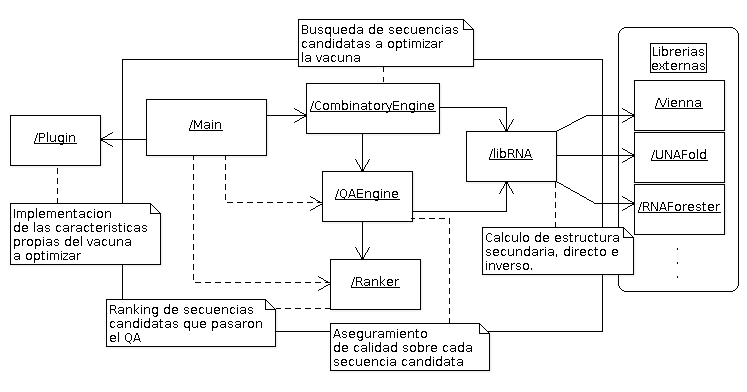
\includegraphics[scale=0.5]{architecture.png}
  \caption{Arquitectura de vac-o.}
\label{arquitectura}
\end{figure}

\begin{itemize}
   \item \textbf{Main:} Representa el componente principal en t\'erminos de
ejecuci\'on del sistema. Comprende principalmente, la inicializaci\'on y
configuraci\'on de otros componentes.
   \item \textbf{Plugin:} Representa la implementaci\'on de las
caracter\'isticas propias de la vacuna que se desea optimizar. Brinda
informaci\'on para la configuraci\'on inicial como as\'i tambi\'en, los
criterios para evaluar las secuencias candidatas.
   \item \textbf{CombinatoryEngine:} Representa el motor combinatorio del
sistema encargado de encontrar, nuevas secuencias que sean candidatas a
optimizar la atenuaci\'on del virus.
   \item \textbf{QAEngine:} Representa el motor de control de calidad del
sistema encargado de decidir, si una secuencia candidata pasa el control o no.
   \item \textbf{Ranker:} Representa el componente encargado de mantener un
``ranking'' de secuencias que sera adem\'as, el resultado final de la
ejecuci\'on.
   \item \textbf{libRNA:} Representa el componente que provee al sistema
funcionalidades para la manipulaci\'on de secuencias y estructuras de \ac{RNA}
(``folding'' directo e inverso y comparaci\'on estructural, entre otras)
utilizando librer\'ias externas.
  \end{itemize}

En las siguientes secciones profundizaremos sobre los componentes ``libRNA'' y
``CombinatoryEngine'' por ser probablemente los mas importantes en cuanto a sus
responsabilidades y dejaremos como lectura adicional la ``Especificaci\'on de
Dise\~no de Software'' que contiene una descripci\'on detallada de todos los
componentes de la arquitectura presentada. Al mismo tiempo, profundizar sobre
estos componentes, nos permitir\'a introducir los principales patrones de
dise\~no que se utilizaron de forma an\'aloga en los dem\'as.

\section{Librer\'ias externas}

Como vimos en la secciones~\ref{folding} y \ref{inverse}, existen diversas
implementaciones que resuelven el problema de la predicci\'on (directa e
inversa) de estructura secundaria de \ac{RNA} y lo mismo ocurre para el caso de
la comparaci\'on estructural. Adem\'as no se descarta la posibilidad de que en
el futuro aparezcan nuevas y mejores implementaciones. 

Por todo esto, uno de los requerimientos del software fue que sea posible el uso
de cualquiera de estas implementaciones de manera transparente. El problema
radica en que cada librer\'ia tiene diferentes formas de recibir los
par\'ametros de entrada y diferentes formas de dar los resultados que genera. A
ra\'iz de esto se propuso el componente ``libRNA'' como una forma de unificar el
acceso a estas librer\'ias externas e integrarlas al resto del sistema. Las
interfaces propuestas fueron las siguientes:

\begin{itemize}
 \item \textbf{IFold:} Provee la predicci\'on directa (\textit{folding})
de secuencias de \ac{RNA}.
 \item \textbf{IFoldInverse:} Provee la predicci\'on inversa (\textit{inverse
folding}) de secuencias de \ac{RNA}.
 \item \textbf{IStructureCmp:} Provee la comparaci\'on de estructuras
secundarias
de \ac{RNA}.
 \item \textbf{ISequenceCmp:} Provee la comparaci\'on de secuencias de
\ac{RNA}.
\end{itemize}

En esto podemos ver la idea del principio de dise\~no \ac{DIP}. Haciendo que el
sistema dependa de estas interfaces en lugar de sus respectivas
implementaciones logramos abstraer los detalles de cada librer\'ia externa y
logramos un software mas vers\'atil. En el capitulo~\ref{librerias} veremos
algunos detalles sobre las implementaciones de estas interfaces.

\section{Motor combinatorio}

El componente ``CombinatoryEngine'' contiene todo lo referente al recorrido del
espacio de b\'usqueda por lo que es claramente, uno de los componentes
principales de \ac{vac-o}. Esto es fundamentalmente, las regiones
combinatorias y las diferentes estrategias de b\'usqueda.
